%%%%%%%%%%%%%%%%%%%%%%%%%%%%%%%%%%%%%%%%%%%%%%%%%%%%%%%%%%%%%%%%%%%%%%
% Lớp 12 | Ứng dụng đạo hàm để khảo sát hàm số | Khảo sát sự biến thiên và vẽ đồ thị hàm số
% Dạng 2D1?5-4: Sự tương giao của hai đồ thị (liên quan đến tọa độ giao điểm)
% Số câu: 33  (sinh tự động bởi tach_cau.py; từ nay thầy sửa trực tiếp file này)
%%%%%%%%%%%%%%%%%%%%%%%%%%%%%%%%%%%%%%%%%%%%%%%%%%%%%%%%%%%%%%%%%%%%%%

%%%%%%%%%%%%%%%% TRẮC NGHIỆM 4 PHƯƠNG ÁN %%%%%%%%%%%%%%%%

% nguồn: Phan1_Lop_12_Dai_so_Chuong_1
\begin{ex}%[2D1N5-4]%[ma:19a95f9a]
		Đồ thị của hàm số $y=x^3-3x+2$ cắt trục tung  tại điểm có tung độ bằng
	\choice 
			 {$0$}
			{$1$} 
			 {\True $2$}
			{$-2$} 
	\loigiai{ 
			Ta  có $f(0)=2$.\\
			Vậy đồ thị hàm số cắt trục tung tại điểm có  tung độ bằng $2$.
		} 
	\end{ex}

% nguồn: Phan1_Lop_12_Dai_so_Chuong_1
\begin{ex}%[2D1H5-4]%[ma:a7b081ae]
		Cho hàm số $y = x^3 + 3x^2 + mx + m, \left(C_m\right)$. Tìm các giá trị của m để đường thẳng $d$  đi qua $I(-1; 2)$ có hệ số góc bằng $-m$ cắt đồ thị hàm số $\left(C_m\right)$ tại $3$ điểm phân biệt.
	\choice 
			 {\True $m < \dfrac{3}{2}$}
			{$m  > \dfrac{3}{2}$}
			{$m  \leq-2$}
			{$m  > 2$}
	 \loigiai{
			Ta  có phương trình đường thẳng $d\colon y=-mx - m + 2$.\\
			 Xét phương trình hoành độ giao điểm của $d$ và $\left(C_m\right)$:
			 \allowdisplaybreaks
			\begin{eqnarray*}
				 &&x^3 + 3x^2 + mx + m = -mx - m + 2,\qquad(1)\\
				&\Leftrightarrow& x^3+3x^2+2m x+2m-2=0\\ 
				&\Leftrightarrow& (x+1)\left(x^2+2  x+2 m-2\right) = 0\\
				&\Leftrightarrow& \hoac{&x=-1 \\& x^2 + 2x  + 2m - 2 = 0 \qquad(2).}
			\end{eqnarray*}
			Để cho $d$ và $\left(C_m\right)$ cắt nhau tại $3$ điểm phân biệt khi  và chỉ khi $(1)$ có $3$ nghiệm phân biệt
			$\Leftrightarrow(2)$ có hai nghiệm phân biệt  khác $-1\Leftrightarrow\heva{&\Delta'=1-(2m-2) > 0\\& 1-2+2m-2\neq 0} \Leftrightarrow m < \dfrac{3}{2}$.
		} 
	\end{ex}

% nguồn: Phan1_Lop_12_Dai_so_Chuong_1
\begin{ex}%[2D1H5-4]%[ma:efeeb800]
		Số giao điểm của đồ thị  hàm số $y=x^3+3x^2$ và đồ thị hàm số $y=3x^2+3x$ là
	 \choice
			{\True $3$} 
			 {$1$}
			 {$2$}
			{$0$} 
	 \loigiai{
			Phương trình hoành độ giao điểm của hai đồ thị  đã cho là
			\[x^3+3x^2=3x^2+3x \Leftrightarrow x^3-3x=0 \Leftrightarrow \hoac{&  x=0 \\& x=\sqrt {3}\\& x=-\sqrt {3}.} \]
			Hai đồ thị đã cho cắt nhau  tại $3$ điểm.
		 }
	\end{ex}

% nguồn: Phan1_Lop_12_Dai_so_Chuong_1
\begin{ex}%[2D1V5-4]%[ma:0aad2032]
	Cho hàm số $y=2x^3-7x^2+3x$ có đồ thị ($C$) và hàm số $y=x^3-5x^2+(3-m) x+2m$ (với $m \in \mathbb{R}$) có đồ thị $(P)$. Biết đồ thị hàm số $(C)$ cắt $(P)$ tại ba điểm phân biệt có hoành  độ nằm trong $[-2; 4]$. Tổng các giá trị nguyên của $m$ bằng
	\choice 
		 {\True $-6$}
		 {$-10$}
		{$-8$} 
		 {$-5$}
	 \loigiai{
		Xét phương trình hoành độ giao điểm 
		 \[2x^3 - 7x^2 + 3x = x^3 - 5x^2 + (3 - m)x + 2 m \Leftrightarrow x^3 - 2x^2 + mx - 2m = 0. \qquad(1)\]
		Đồ thị hàm số $(C)$ cắt $(P)$ tại ba điểm phân biệt có hoành độ nằm trong $[-2;  4]$ khi và chỉ khi phương trình $(1)$ có $3$ nghiệm phân biệt thuộc $[-2; 4]$.\\
		Ta  có
		$$(1) \Leftrightarrow (x^2 + m)(x - 2) = 0 \Leftrightarrow \hoac{&x = 2 \in [-2; 4]  \\& x^2 + m = 0 .\qquad(2)} $$
		Phương trình  $(1)$ có $3$ nghiệm phân biệt thuộc $[-2; 4] \Leftrightarrow$ Phương trình (2) có hai nghiệm phân biệt thuộc $[-2; 4]$ và khác $2$.\\
		Đặt  $g(x)=x^2+m \Rightarrow g'(x)=2x$, ta có $g'(x)=0\Leftrightarrow x=0$.\\
		Bảng biến  thiên của $y=g(x)$
		\begin{center}
			\begin{tikzpicture}[scale=1,font=\footnotesize,line join=round,line cap=round,>=stealth]
				 \tkzTabInit[nocadre=false,lgt=1.2,espcl=2.5,deltacl=0.6]
					{$x$/0.6,$g'(x)$/0.6,$g (x)$/2} 
					 {$-2$,$0$,$2$,$4$}
				 \tkzTabLine{,-,0,+,t,+}
				 \path
					($(N13)!0.45!(N12)$) node[xshift=10pt] (A1){$m+4$} 
					($(N23)!0.1!(N22)$) node (A2){$m$} 
					($(N33)!0.45!(N32)$) node  (A3){$m+4$}
					 ($(N43)!0.8!(N42)$) node (A4){$m+16$};
				 \foreach \x/\y in {A1/A2,A2/A3,A3/A4}{
					 \draw[-stealth] (\x)--(\y);
				} 
			\end{tikzpicture}
		\end{center}
		Từ bảng biến thiên phương trình $g(x)=0$ có hai nghiệm phân  biệt thuộc $[-2; 4]$ và khác $2$
		$$\Leftrightarrow m < 0< m+4\Leftrightarrow-4<  m < 0.$$
		Vì $m \in \mathbb{Z}$, nên $m \in \{-3;  -2; -1\}$. \\
		Tổng các giá trị nguyên của $m$ bằng $-6$. 
	} 
\end{ex}

% nguồn: Phan1_Lop_12_Dai_so_Chuong_1
\begin{ex}%[2D1V5-4]%[ma:9536de28]
	Tìm các giá trị thực của  tham số $m$ để đồ thị hàm số $y=x^3-3x^2+2$ cắt đường thẳng $y=m(x-1)$ tại ba điểm phân biệt có hoành độ $x_1$, $x_2$, $x_3$ thoả mãn $x_1^2+x_2^2+x_3^2> 5$.
	 \choice
		{$m  \geq-3$}
		 {\True $m >-2$}
		{$m >-3$} 
		{$m \geq-2$} 
	 \loigiai{
		Phương  trình hoành độ giao điểm
		\allowdisplaybreaks 
		\begin{eqnarray*}
			x^3 - 3x^2 + 2 = m(x -  1)
			&\Leftrightarrow&  (x-1)\left(x^2-2 x-2-m\right)=0\\
			&\Leftrightarrow& \hoac{&x =  1 \qquad(*)\\&x^2 - 2x - 2 - m = 0.}
		\end{eqnarray*}
		Đồ thị hàm số $y=x^3-3x^2+2$ cắt đường thẳng $y=m(x-1)$ tại ba điểm  phân biệt khi và chỉ khi phương trình $(*)$ có hai nghiệm phân biệt khác $1\Leftrightarrow\heva{&1+2+m > 0\\& 1-2-2-m \neq 0} \Leftrightarrow m >-3$.\\
		Gọi $x_2$, $x_3$  là hai nghiệm của phương trình $(*)$.\\
		 Ta có $x_1^2+x_2^2+x_3^2> 5\Leftrightarrow\left(x_2+x_3\right)^2-2x_2 x_3 > 4\Leftrightarrow 4-2(-2-m) > 4\Leftrightarrow m >-2$.\\
		Vậy $m >-2$. 
	} 
\end{ex}

% nguồn: Phan1_Lop_12_Dai_so_Chuong_1
\begin{ex}%[2D1V5-4]%[ma:f9a0789e]
	Cho hàm số $y = x^3 - 2x^2 +  (1 - m)x + m$ có đồ thị $(C)$. Tìm tất cả các giá trị thực của tham số $m$ để $(C)$ cắt trục hoành tại $3$ điểm phân biệt $x_1$, $x_2$, $x_3$ sao cho $x_1^2 + x_2^2 + x_3^2 < 3$.
	 \choice
		{\True \def\dotEX{$\heva{& 
		-\dfrac{1}{4} <  m < \dfrac{1}{2}\\&
		m  \ne 0.}$}}
		{$m <  1$}
		{$\dfrac{1}{4} < m  < \dfrac{1}{2}$}
		{$\dfrac{1}{4} < m  < 1$}
	 \loigiai{
		Phương  trình hoành độ giao điểm
		\begin{eqnarray*}
			& & x^3 - 2x^2 + (1 - m)x + m = 0\\ &\Leftrightarrow& (x - 1)(x^2 - x - m) =  0\\
			&\Leftrightarrow& \hoac{&x=1\\&x^2-x-m=0.\quad \quad \hfill(1)} 
		\end{eqnarray*}
		Không mất tính tổng quát, đặt $x_3 = 1$ là một nghiệm của phương trình.\\ 
		Để $(C)$ cắt trục hoành tại $3$ điểm phân biệt thì phương  trình
		 $
		x^2 - x - m =  0$
		 có hai nghiệm phân biệt khác $1$
		 $\Leftrightarrow
		\heva{ 
		 &m \ne 0\\
		&\Delta = 1 + 4m > 0 \Leftrightarrow m  > -\dfrac{1}{4}
		} 
		 $.\\
		Gọi hai nghiệm của phương trình $(1)$ là  $x_1$, $x_2$.\\
		Theo định  lý Vi-ét ta có $\heva{&x_1+x_2=1\\&x_1\cdot x_2=-m.}$\\
		Do đó 
		\begin{eqnarray*}
			& & x_1^2 + x_2^2 + x_3^2 < 3 \\ 
			&\Leftrightarrow& x_1^2 + x_2^2 <  2 \\
			 &\Leftrightarrow& (x_1 + x_2)^2 - 2x_1\cdot x_2 < 2 \\
			&\Leftrightarrow& 1^2 + 2m < 2  \Leftrightarrow m < \dfrac{1}{2}.
		\end{eqnarray*}
		 Vậy các giá trị thỏa mãn là $\heva{&-\dfrac{1}{4}<m<\dfrac{1}{2}\\&m \ne 0.}$
	 }
\end{ex}


%%%%%%%%%%%%%%%% ĐÚNG/SAI %%%%%%%%%%%%%%%%

% nguồn: Phan1_Lop_12_Dai_so_Chuong_1
\begin{ex}%[2D1H5-4]%[ma:8165844a]
	Cho  hàm số $y=x-\dfrac{1}{x+1}$.
	\choiceTF 
		{Đồ thị của hàm số có tiệm cận đứng là $x=1$} 
		{\True Đồ thị hàm số cắt trục $Oy$ tại $M$. Phương trình tiếp tuyến  của $(C)$ tại $M$ là $y=2x-1$}
		{Tồn  tại hai tiếp tuyến của đồ thị vuông góc với nhau}
		{\True Nếu  đường thẳng $y=k$ cắt $(C)$ tại hai điểm phân biệt $A$ và $B$ sao cho $OA\perp OB$ thì $k$ là nghiệm của phương trình $k^2-k-1=0$}
	 \loigiai{
		\begin{itemchoice}
			\itemch $y=x-\dfrac{1}{x+1}$. Tập xác định $\mathbb{D}=\mathbb{R}\setminus\{-1\}$.\\ 
			Đạo hàm $y'=1+\dfrac{1}{(x+1)^2}>0,\forall x\in \mathbb{D}$ do đó hàm số luôn luôn đồng biến, không có cực đại,  cực tiểu.\\
			$\lim\limits_{x\to-1^\pm}y=\pm\infty$ nên đường thẳng $x=-1$  là tiệm cận đứng.\\
			$\lim\limits_{x\to\pm\infty}y=x$ nên đường thẳng $y=x$  là tiệm cận xiên.\\
			Bảng biến thiên 
			\begin{center}
\begin{tikzpicture}[>=stealth]
		 \tkzTabInit[nocadre=false,lgt=1,espcl=2,deltacl=0.5]{$x$/.7,$y'$/.7,$y$/2}
			 {$-\infty$,$1-\sqrt{2}$,$1$,$1+\sqrt{2}$,$+\infty$}
		\tkzTabLine{,-,$0$,+,d,+,$0$,-,} 
		\tkzTabVar{+/$+\infty$,-/$4$,+D-/$+\infty$/$-\infty$,+/$-4$,-/$-\infty$} 
	\end{tikzpicture}
			\end{center}
			\itemch $M(0;-1), y'(0)=2$. Phương trình tiếp tuyến $(T)$  tại $M$ là $y=2(x-0)-1\Leftrightarrow y=2x-1$.
			\itemch Tiếp  tuyến $(T_1)$ của $(C)$ tại $P(x_1; y_1)$ có hệ số góc $k_1=y'(x_1)=1+\dfrac{1}{(x_1+1)^2}>0$.\\
			Tiếp tuyến $(T_2)$ của $(C)$ tại $Q(x_2; y_2)$ có  hệ số góc $k_2=y'(x_2)=1+\dfrac{1}{(x_2+1)^2}>0$.\\
			Do $y'(x_1)>0$, $y'(x_2)>0$ nên không  thể có 2 tiếp tuyến của $(C)$ vuông góc nhau.
			\itemch $y=x-\dfrac{1}{x+1}=\dfrac{x^2+x-1}{x+1}$.\\ 
			 Phương trình hoành độ giao điểm của $(C)$ và đường thẳng $y=k$.\\
			$\dfrac{x^2+x-1}{x+1}=k\Leftrightarrow\heva{&x \ne -1  \\&x^2 - (k-1)x - (k+1) = 0 \quad (*)}$.\\
			 Phương trình $(*)$ có 2 nghiệm phân biệt $x_A, x_B\neq-1$ và
			$\heva{&x_A + x_B=k-1\\&x_A\cdot x_B=-(k+1)}$ và $A(x_A;k)$,  $B(x_B;k)$.\\
			 Ta có $\overrightarrow{OA}=(x_A,k)$, $\overrightarrow{OB}=(x_B,k)$.\\
			$\overrightarrow{OA} \perp \overrightarrow{OB} \Leftrightarrow \overrightarrow{OA} \cdot \overrightarrow{OB} = 0 \Leftrightarrow x_A x_B + k^2  = 0 \Leftrightarrow -k - 1 + k^2 = 0 \Leftrightarrow
			\hoac{&k=\dfrac{1-\sqrt{5}}{2}\\&k=\dfrac{1+\sqrt{5}}{2}.}$\\ 
			Thử lại,  $k=\dfrac{1-\sqrt{5}}{2}$ và $k=\dfrac{1+\sqrt{5}}{2}$ đều thỏa mãn yêu cầu bài toán.
		\end{itemchoice}
	} 
\end{ex}

% nguồn: Phan1_Lop_12_Dai_so_Chuong_1
\begin{ex}%[2D1H5-4]%[ma:0f265bf7]
	 \immini{
	Cho  hàm số $f(x)=ax^3+bx^2+cx+d$ có đồ thị như hình sau đây
	\choiceTF 
		 {\True Giá trị cực tiểu của hàm số $f(x)$ bằng $-1$}
		{\True Phương trình $\log_3\left(f(x)+6\right)=2$ có  $2$ nghiệm}
		{Hàm số  $y=f(x)$ đồng biến trên khoảng $(1;3)$}
		 {\True Tổng $2025a+b+c+d=-2023$}
		 }
		 {\resizebox{!}{5cm}{
		\begin{tikzpicture}[line join=round,line cap=round,>=stealth]
			 \draw[->] (-1.5,0) -- (4.5,0) node[above]{$x$};
			\draw[->] (0,-2.0) --  (0,5) node[left]{$y$};
			\draw (0,0)  circle (1pt) node[above right]{$O$};
			\draw[samples=150,smooth,domain=-1.17:3.1]  plot (\x,{-1*(\x)^3+3*(\x)^2+0*(\x)-1});
			\draw[dashed] (0,3)-|(2,0); 
			\foreach \x in  {-1,1,2,3,4}
			\draw[shift={(\x,0)}] (0,1pt)--(0,-1pt)  node[below]{$ \x $};
			 \foreach \y in {-2,-1,1,2,3,4}
			\draw[shift={(0,\y)}]  (1pt,0)--(-1pt,0) node[left]{$ \y $};
		\end{tikzpicture}
		} 
		 }
	 \loigiai{
		\begin{itemchoice}
			 \itemch
			Dựa vào đồ thị  hàm số ta thấy giá trị cực tiểu của hàm số $f(x)$ bằng $-1$.
			 \itemch
			Ta  có: $\log_3\left(f(x)+6\right)=2\Leftrightarrow f(x)+6=9\Leftrightarrow f(x)=3 (*)$.\\
			Số nghiệm của phương trình $(*)$ là~số giao điểm của đồ  thị hàm số $y=f(x)$ với đường thẳng.\\
			$y=3$.  Dựa vào đồ thị ta thấy phương trình $(*)$ có $2$ nghiệm.
			\itemch 
			Dựa  vào đồ thị ta thấy hàm số $y=f(x)$ đồng biến trên khoảng $(1;2)$ và nghịch biến trên khoảng $(2;3)$.
			 \itemch
			Ta có:  $f’(x)=3ax^2+2bx+c$.\\
			Theo giả thiết ta có: $\heva{&f’(0)=0\\&f’(2)=0\\&f(0)=-1\\&f(2)=3}\Leftrightarrow\heva{&c=0\\&12a+4b+c=0\\&d=-1\\&8a+4b+2c+d=3}\Leftrightarrow\heva{&a=-1\\&b=3\\&c=0\\&d=-1.}$ \\ 
			Tổng  $2025a+b+c+d=-2025+3+0-1=-2023$.
		\end{itemchoice}
	} 
\end{ex}

% nguồn: Phan1_Lop_12_Dai_so_Chuong_1
\begin{ex}%[2D1H5-4]%[ma:2f12f4ef]
	Cho hàm số bậc ba  $y=f(x)=a x^3+b x^2+c x+d$ có đồ thị như hình vẽ. Khi đó
	\immini{ \choiceTF 
	{Hàm  số đạt cực tiểu tại $x=-1$}
	 {\True Hàm số nghịch biến trên khoảng $(0; 1)$}
	{\True  Phương trình $2f(x)+1=0$ có 3 nghiệm phân biệt}
	{\True $f(5)=111$}}{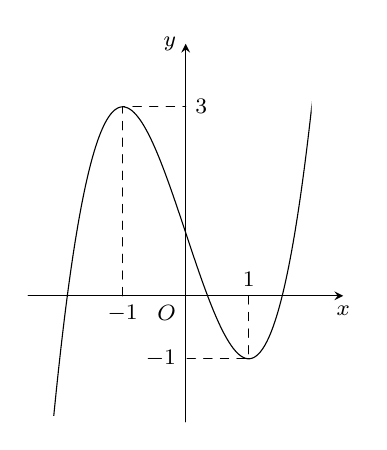
\begin{tikzpicture}[scale=0.8,>=stealth,font=\footnotesize,line join=round,line cap=round]
		 \def\a{1} \def\b{0} \def\c{-3} \def\d{1}
		\def\xmin{-2.5}  \def\xmax{2.5}
		 \def\ymin{-2} \def\ymax{4}
		\draw[->] (\xmin,0)--(\xmax,0) node  [below]{$x$};
		\draw[->] (0,\ymin)--(0,\ymax) node [left]{$y$}; 
		\node at  (0,0) [below left]{$O$};
		 \node at (0,3) [right]{$3$};
		\node at (0,-1)  [left]{$-1$};
		\node at (-1,0) [below]{$-1$}; 
		\node at (1,0)  [above]{$1$};
		 \draw[dashed] (1,0)--(1,-1)--(0,-1);
		\draw[dashed] (-1,0)--(-1,3)--(0,3); 
		\clip (\xmin+0.1,\ymin+0.1)  rectangle (\xmax-0.5,\ymax-0.1);
		 \draw[smooth,samples=300] plot (\x,{\a*(\x)^3+\b*(\x)^2+\c*(\x)+\d});
	\end{tikzpicture}
	 }
	\loigiai{ 
		\begin{itemchoice}
			\itemch Sai. Hàm số đạt cực tiểu tại $x=-1$. Từ  đồ thị ta có $x_{text{CT}}=1$.
			\itemch Đúng. Hàm số nghịch biến trên  khoảng $(0; 1)$.
			\\Hàm số nghịch biến  trên khoảng $(-1; 1)$. Do đó hàm số nghịch biến trên khoảng $(0; 1)$.
			\itemch Đúng. Ta có  $2f(x)+1=0\Leftrightarrow f(x)=\dfrac{-1}{2}$.\\
			Do đường thẳng $y=-\dfrac{1}{2}$ cắt đồ thị hàm số $y=f(x)$ tại 3 điểm phân biệt nên phương trình $2f(x)+1=0$ có 3  nghiệm phân biệt.\\
			\itemch Đúng.  Ta có $f'(x)=3a x^2+2b x+c$.\\
			Vì đồ thị hàm  số có điểm cực đại $(-1; 3)$ và điểm cực tiểu $(1;-1)$ nên
			$$\heva{&f (-1)=3  \\
			&f (1)=-1 \\ 
			&f(-1)=0\\ 
			 &f'(1)=0}\Leftrightarrow
			 \heva{&-a+b-c+d=3 \\
			 &a+b+c+d=-1 \\
			&3a-2b+c=0 \\ 
			&3a+2b+c=0}\Leftrightarrow \heva{&a=1\\ 
			 &b=0\\
			&c=-3\\ 
			 &d=1.}$$
			Hay $f(x)=x^3-3x+1$. Khi đó  $f(5)=111$.
		\end{itemchoice}
	} 
\end{ex}

% nguồn: Phan1_Lop_12_Dai_so_Chuong_1
\begin{ex}%[2D1V5-4]%[ma:683ced72]
	Cho hàm  số $f(x)=\left(\dfrac{1}{2}\right)^{x}$.
	\choiceTF 
		 {\True Phương trình $f(x)=1$ có một nghiệm là $x=0$}
		{Bất phương trình $f(x) \geq  1$ có tập nghiệm là $[0;+\infty)$}
		{Điều kiện của tham số $m$ để phương trình $f(x)=m$ có nghiệm là $m \geq 0$} 
		{\True Tích các nghiệm  của phương trình $2^{x^2-x} \cdot f(x)=3$ bằng $-\log _2 3$}
	 \loigiai{
		\begin{itemchoice}
			\itemch 
			Ta có  $f(x)=1 \Leftrightarrow\left(\dfrac{1}{2}\right)^{x}=1 \Leftrightarrow x=0$.
			\itemch Ta có $$f(x) \geq 1 \Leftrightarrow\left(\dfrac{1}{2}\right)^{x} \geq 1 \Leftrightarrow\left(\dfrac{1}{2}\right)^{x} \geq\left(\dfrac{1}{2}\right)^{0} \Leftrightarrow x \leq 0.$$ Suy ra bất phương trình có tập  nghiệm $S=(-\infty;0]$.
			\itemch Phương trình $f(x)=m \Leftrightarrow\left(\dfrac{1}{2}\right)^{x}=m$  có nghiệm khi $m>0$.
			\itemch  Ta có \allowdisplaybreaks
			\begin{eqnarray*}
				2^{x^2-x} \cdot f(x)=3  &\Leftrightarrow& 2^{x^2-x} \cdot\left(\dfrac{1}{2}\right)^{x}=3 \\&\Leftrightarrow& 2^{x^2-2x}=3 \Leftrightarrow x^2-2x-\log _{2} 3=0.
			\end{eqnarray*}
			Suy ra tích các nghiệm của phương trình là $$x_1\cdot  x_2=\dfrac{-\log _2 3}{1}= -\log _2 3.$$
		\end{itemchoice}
	} 
\end{ex}

% nguồn: Phan1_Lop_12_Dai_so_Chuong_1
\begin{ex}%[2D1V5-4]%[ma:e0b4e875]
	Cho hàm số $f(x)=\dfrac{2x-1}{x^2+2}$. 
	\choiceTF 
		{\True Đồ thị hàm số $y=f(x)$ nhận trục hoành làm tiệm cận ngang} 
		{Hàm số $f(x)$ có $x=2$ là điểm cực tiểu} 
		{\True Với mọi $x \in \mathbb{R}$, ta luôn có $-1 \leq f(x) \leq \dfrac{1}{2}$} 
		{Nếu $-1<m \leq 0$ thì phương trình  $f(x)=m$ có hai nghiệm}
	 \loigiai{
		\begin{itemchoice}
			 \itemch
			\begin{itemize}
				\item  Tập xác định $\mathscr{D}=\mathbb{R}$.
				\item Ta có $\lim\limits_{x\to-\infty}f(x)=0$, $\lim\limits_{x\to+\infty}f(x)=0$ suy ra $y=0$ là tiệm cận ngang của đồ thị hàm số $f(x)$ hay đồ thị hàm  số $y=f(x)$ nhận trục hoành làm tiệm cận ngang.
				 \item $f'(x)=\dfrac{-2\left(x^2-x-2\right)}{\left(x^2+2\right)^2}$;\\
				$f'(x)=0\Leftrightarrow -2\left(x^2-x-2\right)=0 \Leftrightarrow \hoac{& x=-1 \\ &  x=2.}$
				 \item Bảng biến thiên
				\begin{center}
					
\begin{tikzpicture}
						\tkzTabInit[espcl=3.2,lgt=1.5,nocadre] 
						 {$x$/0.7,$f'(x)$/0.7,$f (x)$/2.1}
						{$-\infty$,$-1$,$2$,$+\infty$} 
						 \tkzTabLine{,-,0,+,0,-,}
						\tkzTabVar{+/$0$,-/$-1$,+/$\dfrac{1}{2}$,-/$0$} 
					\end{tikzpicture}
				\end{center}
			\end{itemize}
			\itemch Hàm số $f(x)$ có $x=2$  là điểm cực đại.
			\itemch Dựa vào bảng  biến thiên ta có $-1 \leq f(x) \leq \dfrac{1}{2}$ với mọi $x \in \mathbb{R}$.
			\itemch Khi $m=0$, phương trình $f(x)=m \Leftrightarrow \dfrac{2x-1}{x^2+2} =0 \Leftrightarrow 2x-1=0\Leftrightarrow  x=\dfrac{1}{2}$ chỉ có một nghiệm.
		\end{itemchoice}
	 }
\end{ex}

% nguồn: Phan1_Lop_12_Dai_so_Chuong_1
\begin{ex}%[2D1V5-4]%[ma:a0a89b62]
	Cho hàm số $f( x)=a{{x}^{4}}+b{{x}^{2}}+c$ có đồ thị là đường cong trong hình bên. 
	\begin{center}
		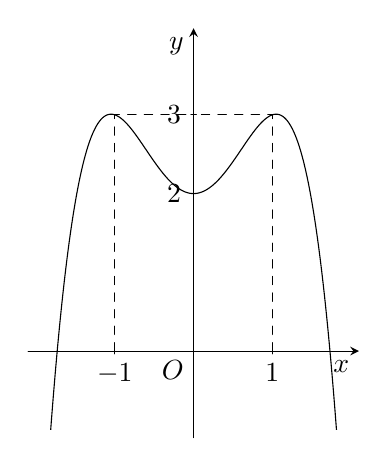
\begin{tikzpicture}[line join=round,line cap=round,>=stealth]
			 \tikzset{ethicknode/.style={scale=0.9}}
			\draw[->]  (-2.1,0)--(2.1,0) node[below left] {$x$};
			\draw[->] (0,-1.1)--(0,4.1) node[below left] {$y$}; 
			 \draw (0,0) node [below left] {$O$};
			\foreach \x/\nx  in {-1/-1,1/1}
			\draw[thin] (\x,1pt)--(\x,-1pt) node  [below] {$\nx$};
			\foreach \y/\ny in {2/2,3/3} 
			\draw[thin] (1pt,\y)--(-1pt,\y)  node [left] {$\ny$};
			 \draw[dashed,thin](-1,0)--(-1,3)--(0,3);
			\draw[dashed,thin](1,0)--(1,3)--(0,3); 
			\begin{scope}
				\clip  (-2,-1) rectangle (2,4);
				\draw[samples=200,domain=-2:2,smooth,variable=\x] plot (\x,{-5/6*((\x)^4)+0*((\x)^3)+11/6*((\x)^2)+0*(\x)+2}); 
			\end{scope}
		\end{tikzpicture}
	\end{center}
	 \choiceTF
		{\True Đồ thị của hàm  số cắt trục hoành tại 2 điểm phân biệt}
		{\True Số nghiệm thực của phương trình $f\left( x  \right)=1$ là 2}
		{Số nghiệm  thực của phương trình $f\left( x \right)=\dfrac{3}{2}$ là 3}
		{\True Phương trình $f\left( x  \right)-3=0$ có tổng các nghiệm bằng 0}
	 \loigiai{
		\begin{itemchoice}
			\itemch 
			 \itemch Vì đường thẳng $y=1$ cắt đồ thị tại 2 điểm nên $f\left( x \right)=1$ có 2 nghiệm.
			\itemch Vì đường thẳng $y=\dfrac{3}{2}$ cắt đồ thị  tại 2 điểm nên $f\left( x \right)=\dfrac{3}{2}$ có 2 nghiệm.
			\itemch Vì đường thẳng $y=3$ cắt đồ thị tại 2 điểm $x_1=-1$, $x_2=1$ nên $f\left( x \right)-3=0$ có tổng các nghiệm bằng 0. 
		\end{itemchoice}
	} 
\end{ex}

% nguồn: Phan1_Lop_12_Dai_so_Chuong_1
\begin{ex}%[2D1V5-4]%[ma:40d89d61]
	Cho hàm số $y=f(x)=x^3-3m^2 x+2024$ có đồ thị $(C)$. 
	\choiceTF 
		{Đồ thị $(C)$ luôn có hai điểm cực trị} 
		{\True Khi $m$ thay đổi thì đồ thị $(C)$ luôn có tâm đối xứng cố định} 
		{\True Khi  $m$ thay đổi thì đồ thị $(C)$ luôn cắt trục hoành tại ít nhất $1$ điểm}
		{\True Khi $(C)$ có $2$ cực trị thì  đường thẳng đi qua $2$ điểm cực trị có dạng $y = ax + b$. Đặt $S = a + b$ thì $S \leq 2024$}
	\loigiai{ 
		\begin{itemchoice}
			\itemch Ta có 
			$y'=3x^2-3m^2$.\\ 
			Hàm số có hai điểm cực trị $\Leftrightarrow $ phương trình  $3x^2-3m^2=0$ có hai nghiệm phân biệt $$\Leftrightarrow m^2>0\Leftrightarrow m\ne 0.$$
			\itemch Ta có 
			$$  y''=0\Leftrightarrow 6x=0\Leftrightarrow x=0\Rightarrow y=2024.$$
			Do đó, khi $m$ thay đổi đồ thị  hàm số luôn có tâm đối xứng là $I(0;2024)$.
			 \itemch Đồ thị hàm bậc ba luôn cắt trục hoành ít nhất một điểm, nên khi $m$ thay đổi, đồ thị luôn cắt trục hoành ít nhất một điểm.
			\itemch Ta  có $ y=\dfrac{1}{3}x\cdot y'+(-2m^2x+2024)$.\\
			Gọi tọa độ hai điểm cực trị  lần lượt là $A(x_1;y_1)$, $B(x_2;y_2)$, trong đó $\heva{&y'(x_1)=0\\&y'(x_2)=0.}$\\
			Mặt khác $A$, $B\in (C)$ do đó 
			$$\heva{&y_1=\dfrac{1}{3}x_1\cdot  y'(x_1)+(-2m^2x_1+2024)\\&y_2=\dfrac{1}{3}x_1\cdot y'(x_2)+(-2m^2x_2+2024)}\Leftrightarrow\heva{&y_1=-2m^2x_1+2024\\&y_2=-2m^2x_2+2024.}$$
			Do đó đường thẳng  đi qua hai điểm cực trị $A$, $B$ có dạng
			$$ y = -2m^2x + 2024 \Rightarrow S =  a + b = -2m^2 + 2024 < 2024\le 2024.$$
		\end{itemchoice}
	} 
\end{ex}

% nguồn: Phan1_Lop_12_Dai_so_Chuong_1
\begin{ex}%[2D1V5-4]%[ma:3e05a605]
	Xét hàm số  $y = \dfrac{\sin x}{1 + \cos x}$ trên khoảng $(0; \pi)$. Khi đó
	\choiceTF 
		{Hàm số nghịch  biến trên khoảng $(0; \pi)$}
		{\True Hàm số  có $2$ điểm cực trị}
		{\True Giá trị  cực tiểu của hàm số là~$\dfrac{5\pi}{24} - \dfrac{2 + \sqrt{3}}{4}$}
		{Đồ thị hàm số $y =f'(x)$ cắt đồ thị hàm số $y = -\dfrac{\sin ^2 x x}{2}$ tại $2$  điểm trên khoảng $(0; \pi)$}
	 \loigiai{
		\textbf{Phương  pháp:}\\
		a),  b), c) Tính đạo hàm và giải phương trình lượng giác từ đó lập bảng biến thiên và kết luận cực trị, sự đồng biến nghịch biến.\\
		d) Giải phương trình hoành độ  giao điểm $f'(x)=-\dfrac{\sin^2 2x }{2}$.\\
		\textbf{Cách giải:} 
		\begin{itemchoice}
			\itemch $y' = \dfrac{1}{2} - 2\sin  x \cos x = 0 \Leftrightarrow \sin 2x = \dfrac{1}{2}
			\Leftrightarrow 
			 \hoac{&2x = \dfrac{\pi}{6} + k2\pi\\&
			2x = \dfrac{5\pi}{6} + k2\pi}\Leftrightarrow \hoac{&x =  \dfrac{\pi}{12} + k\pi\\& x = \dfrac{5\pi}{12} + k\pi.} $\\
			Do $0  < x < \pi$ nên $x=\dfrac{\pi}{12}$, $x = \dfrac{5\pi}{12}$.\\
			Bảng biến  thiên:
			\begin{center}
				\begin{tikzpicture}
					\tkzTabInit[nocadre,lgt=0.8,espcl=2.1] 
						{$x$  /1,$y'$ /0.6,$y$ /2}
						 {$0$,$\dfrac{\pi}{12}$,$\dfrac{5\pi}{12}$,$\pi$}
					\tkzTabLine{,+,$0$,-,$0$,+,} 
					\tkzTabVar{-/,+/$y_\text{  CĐ}$,-/$y_\text{ CT}$,+/}
				\end{tikzpicture}
			\end{center}
			Dựa  vào bảng biến thiên ta thấy hàm số đồng biến trên $\left(\dfrac{5\pi}{12};\pi\right)$.
			\itemch Hàm số có hai  điểm cực trị.
			\itemch Giá trị cực tiểu là~$y_\text{ CT}  = \dfrac{5\pi}{24} - \dfrac{2 + \sqrt{3}}{4}$
			\itemch Ta có 
			\begin{eqnarray*}
				&&  f'(x) = \dfrac{-\sin^2 2x}{2}\\
				&\Leftrightarrow& \dfrac{1}{2} -\sin 2x  = \dfrac{\sin^2 2x}{2}\\
				&\Leftrightarrow& \dfrac{\sin^2 2x}{2}  +\sin 2 x \dfrac{1}{2}=0 \\
				&\Leftrightarrow& \sin 2x = 1 \\ 
				&\Leftrightarrow& 2x =  \dfrac{\pi}{2} + k2\pi\\
				&\Leftrightarrow& x  = \dfrac{\pi}{4} + k\pi,\, k\in\mathbb{Z}.
			\end{eqnarray*}
			Có $0 < x < \pi \Rightarrow 0 < \dfrac{\pi}{4} + k\pi < \pi \Rightarrow x =  \dfrac{\pi}{4} \Rightarrow$ Có $1$ nghiệm trên khoảng $(0; \pi).$
		\end{itemchoice}
	 }
\end{ex}


%%%%%%%%%%%%%%%% TRẢ LỜI NGẮN %%%%%%%%%%%%%%%%

% nguồn: Phan2_Lop_12_Dai_so_Chuong_1
\begin{bt}%[2D1N5-4]%[ma:71ab8706]
	Biết đường thẳng $y=-2x+2$ cắt đồ thị hàm số $y=x^{3}+x+2$ tại điểm duy nhất có tọa độ là $\left( x_{0};y_{0}\right)$.  Tính giá trị của biểu thức $T=x_{0}-y_{0}$.
	\shortans{-2} 
	\loigiai{ 
		Phương trình hoành độ giao điểm là $-2x+2=x^{3}+x+2\Leftrightarrow x^{3}+3x=0\Leftrightarrow x=0\Rightarrow  y=2$. \\
		Vậy tọa độ giao điểm là $\left( 0;2 \right)$  \\
		 Khi đó, $T=0-2=-2$.
	} 
\end{bt}

% nguồn: Phan2_Lop_12_Dai_so_Chuong_1
\begin{bt}%[2D1V5-4]%[ma:68f69b1b]
	 Cho hàm số $y=\dfrac{2x-1}{x+1}$ có đồ thị $(C)$ và điểm $P(2; 5)$. Có bao nhiêu giá trị của tham số $m$ để đường thẳng $d: y=-x+m$ cắt đồ thị $(C)$ tại hai điểm phân biệt $A$ và $B$ sao cho tam giác $PAB$ đều.
	\shortans{2} 
	 \loigiai{
		\begin{center}
			\begin{tikzpicture}[>=latex,line join=round,line cap=round,scale=0.7]
				 \draw[->] (-4,0)--(4,0) node[below]{$x$};
				\draw[->] (0,-2)--(0,6)  node[right]{$y$};
				\draw[red,dashed]  (-1,-2)--(-1,6)
					 (-4,2)--(4,2);
				\foreach \x in  {-3,-2,-1,1,2,3}
				\draw[fill] (\x,0) circle (1pt) node[below]{$\x$}; 
				\foreach \y  in {-1,1,2,3,4,5}
				\draw[fill] (0,\y) circle (1pt)  node[left]{$\y$};
				\clip (-7,-6) rectangle (6,6); 
				 \draw[samples=200,smooth,blue,line width=1] plot[domain=-4:-1.1] (\x,{(2*(\x)-1)/(\x+1)});
				\draw[samples=200,smooth,blue,line width=1] plot[domain=-0.3:4] (\x,{(2*(\x)-1)/(\x+1)}); 
				\draw (0,0)  node[above left]{$O$};
				\draw [dashed] (0,5)--(2,5)--(2,0); 
				 \draw (2,5) circle (1pt) node[above right]{$P$};
			\end{tikzpicture}
		\end{center}
		Hoành độ giao điểm của $d$ và $(C)$ là nghiệm của  phương trình $\dfrac{2x-1}{x+1}=-x+m$.\\
		 $\Leftrightarrow\heva{&x\neq-1\\&2x-1=(-x+m)(x+1)}\Leftrightarrow x^2-(m-3)x-m-1=0\, (1)$.\\
		Ta có $\triangle_{(1)}=(m-3)^2+4(m+1)=m^2-2m+13=(m-1)^2+12>0, \forall m\in\mathbb{R}$ nên $(1)$ luôn có hai nghiệm phân biệt hay $d$ luôn cắt $(C)$ tại  hai điểm phân biệt.\\
		Gọi  $x_1, x_2$ là hai nghiệm phân biệt của $(1)$.\\
		Khi đó tọa độ giao điểm của $d$ và $(C)$  là $A(x_1; -x_1+m), B(x_2; -x_2+m)$.\\
		Tọa độ trung điểm $I$ của $AB$ là  $I=\left(\dfrac{x_1+x_2}{2}; \dfrac{-(x_1+x_2)+2m}{2}\right)=I\left(\dfrac{m-3}{2}; \dfrac{m+3}{2}\right)$.\\
		Ta có $\overrightarrow{PI}=\left(\dfrac{m-7}{2}; \dfrac{m-7}{2}\right)$, vectơ chỉ phương của đường thẳng $d$  là $\vec{u}_{d}=(1; -1)$.\\
		Dễ thấy $\vec{u}_d\cdot\overrightarrow{PI}=0$  nên $P\equiv I$ hoặc $PI\perp d$.\\
		Như vậy hoặc $P\equiv I$ (khi đó $P, A, B$ thẳng hàng) hoặc tồn tại tam giác $PAB$  luôn cân tại $P$.\\
		Khi đó $\triangle PAB$ tồn tại và đều khi và chỉ khi 
		\begin{align*}
			 &\, PI=AB\dfrac{\sqrt{3}}{2}\Leftrightarrow 8\left(\dfrac{m-7}{2}\right)^2=3\left[2(x_1-x_2)^2\right]\Leftrightarrow (m-7)^2=3\left[(x_1+x_2)^2-4x_1x_2\right]\\
			\Leftrightarrow&\, (m-7)^2=3\left[(m-3)^2+4(m+1)\right]\Leftrightarrow  m^2+4m-5=0\Leftrightarrow\hoac{&m=1\\&m=-5.}
		\end{align*}
		Vậy $m\in\{-5;1\}$. 
	} 
\end{bt}

% nguồn: Phan2_Lop_12_Dai_so_Chuong_1
\begin{bt}%[2D1V5-4]%[ma:1ef8f57b]
	Biết rằng có hai giá $m_1, m_2$ của tham số $m$ để đường thẳng $d: y=m-x$ và đồ thị  hàm số $y=\dfrac{x}{x-1}$ có đúng một điểm chung. Tính giá trị của biểu thức $T=m_1+m_2$.
	 \shortans{4}
	\loigiai{ 
		 Điều kiện: $x\neq1$.\\
		Xét phương  trình hoành độ giao điểm \[\dfrac{x}{x-1}=m-x\Leftrightarrow x^2-mx+m=0\quad (1).\]
		Đồ thị hàm số và đường thẳng $d$ có một điểm chung khi và chỉ khi phương trình $(1)$ có nghiệm duy nhất khác  $1$.\\
		\[\Leftrightarrow\heva{&\triangle=0\\&1^2-m\cdot1+m\neq0}\Leftrightarrow  m^2-4m=0\Leftrightarrow\hoac{&m=0\\&m=4.}\]
		 Khi đó $T=m_1+m_2=0+4=4$.
	 }
\end{bt}

% nguồn: Phan2_Lop_12_Dai_so_Chuong_1
\begin{bt}%[2D1V5-4]%[ma:fe019a6a]
	Có bao nhiêu giá trị nguyên của tham  số thực $m$ để đường thẳng $y = 3x + m - 2$ cắt đồ thị $y = (x - 1)^3$ tại ba điểm phân biệt?
	 \shortans{3}
	 \loigiai{
		Phương trình hoành độ giao điểm của hai  đồ thị
		\begin{eqnarray*}
			& &3x + m - 2 = (x - 1)^3\\ 
			& \Leftrightarrow & m = x^3  - 3x^2 + 1.\quad \quad \hfill (1)
		\end{eqnarray*}
		\textit{Nhận xét}: Phương trình $(1)$ là phương trình hoành độ giao điểm của đường thẳng $(d)\colon y = m$ và đồ thị $(C)\colon y = x^3 - 3x^2 +  1$.\\
		Xét hàm số $y = x^3 - 3x^2 + 1$.\\ 
		Ta có  $y' = 3x^2 - 6x$.\\
		$$y' = 0\Leftrightarrow 3x^2 - 6x=0\Leftrightarrow \hoac{&x  = 0\\&x = 2.}$$
		\begin{center}
			
\begin{tikzpicture}
				\tkzTabInit[nocadre=false,lgt=1.2,espcl=2.5,deltacl=0.6] 
					 {$x$/1,$y'$/1,$y$/2}
					{$-\infty$,$0$,$2$,$+\infty$} 
				 \tkzTabLine{,+,z,-,z,+,}
				 \tkzTabVar{-/$-\infty$,+/1,-/$-3$,+/$+\infty$}
			\end{tikzpicture}
		\end{center}
		Để phương trình $(1)$ có $3$ nghiệm phân biệt, đường thẳng $y = m$ phải cắt đồ thị $(C)$ tại  $3$ điểm phân biệt, tức là $-3 < m < 1$.\\
		Số giá trị nguyên của $m$ là $3$. 
	} 
\end{bt}

% nguồn: Phan2_Lop_12_Dai_so_Chuong_1
\begin{bt}%[2D1V5-4]%[ma:8dd18840]
	Tìm giá trị nguyên dương của $m$ để đồ thị hàm số $y=\dfrac{2mx+3m-1}{2x-m^2}$ cắt $Oy$ tại điểm có tung độ bằng  $-4$.
	\shortans{1} 
	\loigiai{ 
		Vì đồ thị hàm số cắt trục $Oy$ tại điểm có tung độ bằng  $-4$ nên ta có \[\dfrac{3m+1}{-m^2}=-4\Leftrightarrow\heva{&m\neq0\\&3m+1=4m^2}\Leftrightarrow\heva{&m\neq0\\&\hoac{&m=1\\&m=-\dfrac{1}{4}}}\Leftrightarrow\hoac{&m=1\\&m=-\dfrac{1}{4}.}\]
		Vì  $m$ nguyên dương nên $m=1$.
	 }
\end{bt}

% nguồn: Phan2_Lop_12_Dai_so_Chuong_1
\begin{bt}%[2D1V5-4]%[ma:94ba59e2]
	Với $m$ là một tham số thực  thì đồ thị hàm số $y = x^3 - 2x^2 + x - 1$ và đường thẳng $y = m$ có nhiều nhất bao nhiêu giao điểm?
	 \shortans{3}
	 \loigiai{
		Xét  hàm số $y = x^3 - 2x^2 + x - 1$ có tập xác định $\mathbb{R}$.\\
		 Ta có
		 $$
		y' = 3x^2 - 4x + 1 =  0 \Leftrightarrow \hoac{&x = \dfrac{1}{3}\\& x = 1.}
		 $$
		Lập  bảng biến thiên
		\begin{center}
			
\begin{tikzpicture}
				\tkzTabInit[nocadre=false,lgt=1.5,espcl=2.2,deltacl=0.8] 
					 {$x$/1,$y'$/1,$y$/2}
					{$-\infty$,$\dfrac{1}{3}$,$1$,$+\infty$} 
				\tkzTabLine{,+,z,-,z,+,} 
				\tkzTabVar{-/$-\infty$,+/$-\dfrac{23}{27}$,-/$-1$,+/$+\infty$} 
			\end{tikzpicture}
		\end{center}
		Dựa vào bảng biến thiên, ta thấy đồ thị hàm số có $2$  cực trị, nên đường thẳng $y = m$ có thể cắt đồ thị tại nhiều nhất $3$ điểm.
	 }
\end{bt}

% nguồn: Phan2_Lop_12_Dai_so_Chuong_1
\begin{bt}%[2D1V5-4]%[ma:21ada8a4]
	Có bao nhiêu  giá trị nguyên của tham số $m$ để phương trình $x^3 - 3x^2 - m^2 + 5m = 0$ có ba nghiệm thực phân biệt?
	 \shortans{0}
	 \loigiai{
		Đặt $f(x) = x^3  - 3x^2 - m^2 + 5m$.\\
		Để phương trình có $3$ nghiệm thực phân  biệt $\Leftrightarrow$ Đồ thị hàm số $f(x)$ phải có hai điểm cực trị $x_1, x_2$ sao cho $f(x_1)\cdot f(x_2) < 0$.\\
		Ta có $f'(x) = 3x^2 -  6x$.
		 $$
		f'(x) = 0 \Leftrightarrow 3x^2 - 6x=0\Leftrightarrow \hoac{&  x = 0 \\& x = 2.}
		 $$
		 Ta thấy phương trình $f'(x)=0$ luôn có $2$ nghiệm phân biệt $x_1=0$ và $x_2=2$ nên hàm số luôn có $2$ điểm cực trị $x_1=0$ và $x_2=2$.\\
		Ta  có $
		f(0) =  -m^2 + 5m$, $f(2) = -m^2 + 5m - 4.
		 $\\
		 Khi đó
		$$ 
		f(0) \cdot f(2) < 0 \Leftrightarrow (-m^2 + 5m)(-m^2 + 5m - 4) < 0\Leftrightarrow \hoac{&0  < m < 1\\&
		4 < m < 5.} 
		 $$
		Vậy không có giá trị  nguyên nào của $m$ thỏa mãn.
	} 
\end{bt}

% nguồn: Phan2_Lop_12_Dai_so_Chuong_1
\begin{bt}%[2D1V5-4]%[ma:123fe5d4]
	Tìm $m$ để đường thẳng $y=-2x+m$ cắt đồ thị hàm số $y=\dfrac{x^2+x-1}{x}$ tại hai điểm $A, B$ sao cho trung điểm  đoạn $AB$ thuộc $Oy$.
	 \shortans{1}
	 \loigiai{
		Phương trình hoành  độ giao điểm $3x^2+(1-m)x-1=0$ ($x\ne 0$).\\
		Vì $\Delta =(1-m)^2+12 >0  \forall m \in \mathbb{R}$ nên phương trình có 2 nghiệm phân biệt $x_1$; $x_2$ khác $0$ với mọi $m$.\\
		 Hoành độ trung điểm $I$ của $AB$: $x_I=\dfrac{x_1+x_2}{2}=\dfrac{m-1}{6}$.\\
	Do $I\in Oy\Leftrightarrow x_I=0\Leftrightarrow\dfrac{m-1}{6}=0\Leftrightarrow  m=1$}.\\
\end{bt}

% nguồn: Phan2_Lop_12_Dai_so_Chuong_1
\begin{bt}%[2D1V5-4]%[ma:08aa0de4]
	Có bao nhiêu giá trị  nguyên dương của tham số $m$ để đồ thị hàm số $(C): y=\dfrac{2x+m}{x+1}$ cắt đường thẳng $d: y=1-x$ tại hai điểm phân biệt.
	\shortans{1} 
	 \loigiai{
		Điều  kiện: $x\neq-1$.\\
		Phương trình hoành độ giao điểm  $\dfrac{2x+m}{x+1}=1-x\Leftrightarrow x^2+2x+m-1=0\, (1)$.\\
		Đường thẳng $d$ cắt $(C)$ tại  hai điểm phân biệt khi và chỉ khi $(1)$ có hai nghiệm phân biệt khác $-1$.\\
		 \[\Leftrightarrow\heva{&1-(m-1)>0\\&1-2+m-1\neq0}\Leftrightarrow\heva{&m<2\\&m\neq2}\Leftrightarrow m<2.\]
		Mà $m$ là số nguyên dương nên suy ra  $m=1$.
	 }
\end{bt}

% nguồn: Phan2_Lop_12_Dai_so_Chuong_1
\begin{bt}%[2D1V5-4]%[ma:0c59dfa8]
	Tìm số giá trị của $m$ để đường thẳng $y=-x+m$ cắt đồ thị hàm số  $y=\dfrac{x^2-1}{x}$ tại hai điểm phân biệt $A$, $B$ sao cho $AB=\sqrt{6}$.
	\shortans{2} 
	 \loigiai{
		Tọa độ $A$, $B$  thỏa: $\dfrac{x^2-1}{x}=-x+m\Leftrightarrow 2x^2-mx-1=0,\quad (x\ne 0)\quad(1)$\\
		Ta thấy $a\cdot  c = -2<0$ nên (1) có hai nghiệm thực phân biệt $x_1$, $x_2$ khác $0$ với mọi $m$.\\
		Gọi $A(x_1;y_1)$,  $B(x_2;y_2)$. Do đó $AB^2=(x_1-x_2)^2+(y_1-y_2)^2=2(x_1-x_2)^2$.\\
		Áp dụng định lí Viet cho phương trình $(1)$ ta có được $\heva{&x_1+x_2=\dfrac{m}{2}\\&x_1x_2=-\dfrac{1}{2}.}$\\ 
	$\Rightarrow AB^2=2[(x_1+x_2)^2-4x_1x_2]=\dfrac{m^2}{2}+4, AB=6\Leftrightarrow\dfrac{m^2}{2}+4=6\Leftrightarrow  m=\pm 2$.}
\end{bt}

% nguồn: Phan2_Lop_12_Dai_so_Chuong_1
\begin{bt}%[2D1V5-4]%[ma:6a59c5f9]
	Cho hàm số $y = x^3 - 3x^2 + mx + 1$ có  đồ thị $(C)$ và đường thẳng $d\colon y = 2x + 1$. Có bao nhiêu giá trị nguyên dương của tham số $m$ để $(C)$ cắt $d$ tại $3$ điểm phân biệt?
	\shortans{3} 
	 \loigiai{
		Phương trình hoành độ giao điểm 
		\begin{eqnarray*}
			& & x^3 - 3x^2 + mx + 1 =  2x + 1\\
			 &\Leftrightarrow &x^3 - 3x^2 + (m-2)x = 0\\
			& \Leftrightarrow& x(x^2 -  3x + m - 2) = 0\\
			&\Leftrightarrow& \hoac{&x=0\\&x^2  - 3x + m - 2=0.\quad \hfill(2)}
		\end{eqnarray*}
		Đặt $f(x)=x^2 - 3x  + m - 2$.\\
		Để $(C)$ cắt  $d$ tại $3$ điểm phân biệt thì $(2)$ có hai nghiệm phân biệt khác $0$
		$$\Leftrightarrow 
		\heva{& f(0) = -2 + m  \ne 0\\
		 &
		\Delta = 9 -  4(m-2) > 0} \Leftrightarrow \heva{&m \ne 2\\& -4m + 17 > 0}\\
		\Leftrightarrow \heva{&m  \ne 2\\ &m < \dfrac{17}{4}.}
		$$ 
		Vì $m$ là số nguyên dương nên $m  \in \{1,3,4\}$.\\
		 Vậy có $3$ giá trị nguyên dương của $m$ thỏa mãn.
	 }
\end{bt}

% nguồn: Phan2_Lop_12_Dai_so_Chuong_1
\begin{bt}%[2D1V5-4]%[ma:7476ce10]
	Cho hàm số $y=\dfrac{2x-1}{x-1}$ có đồ thị $(C)$. Tổng các giá trị nguyên dương của tham số $m$ để đường thẳng $d\colon y=x+m$ cắt $(C)$ tại hai điểm phân biệt $A$, $B$ sao cho  $AB=4$.
	 \shortans{3}
	 \loigiai{
		 Điều kiện: $x\neq1$.\\
		Xét phương trình hoành độ  giao điểm $\dfrac{2x-1}{x-1}=x+m\Leftrightarrow x^2+(m-3)x+1-m=0\, (1)$.\\
		Đồ thị $(C)$ cắt $d$ tại hai điểm phân biệt khi và chỉ khi phương trình $(1)$ có hai nghiệm  phân biệt khác $1$.\\
		$\Leftrightarrow \heva{&a\neq0\\&\triangle>0\\&1^2+(m-3)\cdot1+1-m\neq0}\Leftrightarrow\heva{&(m-3)^2-4(1-m)>0\\&-1\neq0}\Leftrightarrow\heva{&m^2-2m+5>0\,\forall m\\&-1\neq0}$\\ 
		Giả sử $x_A, x_B$ là hai  nghiệm của phương trình $(1)$.\\
		Áp dụng định lí  Vi-et, ta có $\heva{&x_A+x_B=3-m\\&x_A\cdot x_B=1-m.}$\\
		Ta có $A(x_A,m)$ và $B(x_B,m)$ nên $AB=4\Leftrightarrow AB^2=16\Leftrightarrow (x_B-x_A)^2+(y_B-y_A)^2=16\Leftrightarrow2(x_B-x_A)^2=16\Leftrightarrow (x_B-x_A)^2=8$.\\ 
		Suy ra  $\left(x_B+x_A\right)^2-4x_Ax_B=8\Rightarrow (3-m)^2-4(1-m)=8\Leftrightarrow m^2-2m-3=0\Leftrightarrow\hoac{&m=-1\\&m=3.}$
		Do $m$ nguyên dương nên $m=3$. 
	 }
\end{bt}

% nguồn: Phan2_Lop_12_Dai_so_Chuong_1
\begin{bt}%[2D1V5-4]%[ma:deb6a17f]
	Cho hàm số $y=\dfrac{(x^2-2x+m)^2-3x-m}{x-3}\quad (C)$ và đường thẳng $(d)\colon y=2x$ ($m$ là tham số thực). Có bao nhiêu giá trị nguyên của $m\in[-15;15]$ để đường thẳng  $(d)$ cắt đồ thị $(C)$ tại bốn điểm phân biệt.
	\shortans{15} 
	\loigiai{ 
		Xét phương trình hoành  độ giao điểm của hai đồ thị hàm số
		\begin{eqnarray}
			\dfrac{(x^2 - 2x + m)^2 - 3x -  m}{x - 3} &=& 2x \nonumber \\
			\Leftrightarrow (x^2 - 2x + m)^2 - 3x - m &=& 2x^2 - 6x \quad  (x \ne 3) \nonumber \\
			\Leftrightarrow (x^2 - 2x + m)^2 &=& 2x^2 - 3x + m  \quad (x \ne 3) \quad \text{ (*)} \nonumber
		\end{eqnarray}
		 Đặt $x^2-2x+m=t$, khi đó ta có\\
		$t^2-t=x^2-x\Leftrightarrow (t^2-x^2)-(t-x)=0\Leftrightarrow  (x-t)(x+t-1)=0\Leftrightarrow \hoac{&t=x\\&t=1-x.}$\\
		Suy ra: $\hoac{&x^2-2x+m=x \\&x^2-2x+m=1-x}$ $ \Leftrightarrow \hoac{&x^2-3x+m=0 \ \ \text{ (1)}  \\&x^2-x+m-1=0 \ \ \text{ (2)}}$\\
		Yêu cầu bài toán $\Leftrightarrow(*)$ phải có 4 nghiệm phân biệt khác $3\Leftrightarrow(1),(2)$ đều phải có hai nghiệm phân biệt khác 3 và các nghiệm của  chúng không trùng nhau. Phương trình (1), (2) đều có hai nghiệm phân biệt khác $3$.
		$\heva{& 9-4m > 0 \\& 3^3-3.3+m \ne 0 \\& 1-4(m-1) > 0 \\& 3^2-3+m-1 \ne 0} 
		 \Leftrightarrow \heva{&m<\dfrac{9}{4}\\&m\ne 0\\&m <\dfrac{5}{4}\\& m\ne-5}
		\Leftrightarrow \heva{& m < 1,25 \\& m \ne 0  \\ & m \ne -5}$\\
		Phương trình (1), (2) không có nghiệm  trùng nhau $\Leftrightarrow$
		 $\heva{&x^2-3x+m = 0 \\&x^2-x+m-1=0}$ (vô nghiệm)\\
		Hệ phương trình 
		$\heva{&2x-1 = 0  \\&x^2-3x+m = 0}$ vô nghiệm $\Leftrightarrow$
		$\heva{&x=\dfrac{1}{2}  \\&x^2-3x+m = 0}$ vô nghiệm\\
		$\Rightarrow\left(\dfrac{1}{2}\right)^2-3.\left(\dfrac{1}{2}\right)+m\ne 0\Leftrightarrow m\ne\dfrac{5}{4}\quad(*)$ 
		Vậy số giá trị nguyên của $m\in[-15;15]$  đồng thời thỏa mãn yêu cầu bài toán là $15$.
	} 
\end{bt}

% nguồn: Phan2_Lop_12_Dai_so_Chuong_1
\begin{bt}%[2D1V5-4]%[ma:a7e88adc]
	Tập hợp các giá trị thực của tham số $m$ để đường thẳng $d: y=x-2m$ cắt đồ thị hàm số $(C): y=\dfrac{x-3}{x+1}$  tại hai điểm phân biệt có hoành độ dương là $(a; b)$. Tính giá trị của biểu thức $T=a+b$.
	 \shortans{1}
	\loigiai{ 
		Xét phương trình hoành độ giao điểm \[x-2m=\dfrac{x-3}{x+1}\Leftrightarrow x^2-2mx+3=0\, (1).\] 
		Đường thẳng $d$ cắt $(C)$ tại hai điểm phân biệt có hoành độ dương khi và  chỉ khi phương trình $(1)$ có hai nghiệm dương phân biệt.\\
		$\Leftrightarrow\heva{&\triangle'=m^2+2m-3>0\\&S=2m>0\\&P=-2m+3>0}\Leftrightarrow\heva{&\hoac{&m<1\\& m>3}\\&m>0\\&m<\dfrac{3}{2}}\Leftrightarrow  0<m<1$.\\
		Khi đó $T=a+b=0+1=1$. 
	 }
\end{bt}

% nguồn: Phan2_Lop_12_Dai_so_Chuong_1
\begin{bt}%[2D1V5-4]%[ma:cafd2f56]
	Cho hàm số $y=\dfrac{x^2+mx-1}{x-1}$ có đồ thị  là $(C)$ ($m$ là tham số thực). Tổng bình phương các giá trị của $m$ để đường thẳng $d: y=m$ cắt đồ thị $(C)$ tại hai điểm $A, B$ sao cho $OA\perp OB$ bằng bao nhiêu?
	 \shortans{3}
	\loigiai{ 
		Phương trình hoành độ giao điểm của đồ thị $(C)$ và đường thẳng $d$ là \[\dfrac{x^2+mx-1}{x-1}=m\Leftrightarrow\heva{&x\neq1\\&x^2+mx-1=mx-m}\Leftrightarrow\heva{&x\neq1\\&g(x)=x^2+m-1=0.}\] 
		Đường thẳng $d: y=m$ cắt đồ thị $(C)$ tại  hai điểm phân biệt khi và chỉ khi $g(x)=0$ có hai nghiệm phân biệt khác $1$, tương đương $$\heva{&\triangle'=1-m>0\\&g(1)\neq0}\Leftrightarrow m\in(-\infty;1)\setminus\{0\}.$$
		Gọi $A(x_1; m), B(x_2; m)$. Khi đó $x_1$, $x_2$ là hai  nghiệm của phương trình $g(x)=0$.\\
		 Theo định lí Vi-ét ta có $\heva{&x_1+x_2=0\\&x_1x_2=m-1.}$\\
		Khi đó $OA\perp OB\Leftrightarrow x_1x_2+m^2=0\Leftrightarrow m^2+m-1=0\Leftrightarrow\hoac{&m=\dfrac{-1+\sqrt{5}}{2}\\&m=\dfrac{-1-\sqrt{5}}{2}}$ (thỏa mãn).\\ 
		Vậy tổng bình phương các giá trị của  $m$ thỏa mãn yêu cầu đề bài là \[\left(\dfrac{-1+\sqrt{5}}{2}\right)^2+\left(\dfrac{-1-\sqrt{5}}{2}\right)^2=3.\]
	 }
\end{bt}

% nguồn: Phan2_Lop_12_Dai_so_Chuong_1
\begin{bt}%[2D1C5-4]%[ma:022a366c]
	Cho hàm số $y = x^3 - (m + 2)x^2 - (2m + 13)x - m - 2$ có đồ thị $(C_m)$; đường thẳng $d\colon y  = mx + m + 8$ và điểm $I(1;4)$. Tính tổng tất cả các giá trị của tham số $m$ biết rằng đường thẳng $d$ cắt đồ thị $(C_m)$ tại ba điểm phân biệt $A$, $B$, $C$ với $A$ có hoành độ bằng $-2$ và tam giác $IBC$ cân tại $I$.
	\shortans{-6} 
	 \loigiai{
		Phương trình hoành độ giao  điểm
		\begin{eqnarray*}
			& &x^3 - (m + 2)x^2 - (2m +  13)x - m - 2 = mx + m + 8\\
			&  \Leftrightarrow&
			x^3  - (m + 2)x^2 - (3m + 13)x - 2m - 10 = 0\Leftrightarrow \hoac{&x=-2\\&x=-1\\&x=m+5.}
		\end{eqnarray*}
		Để đường thẳng $d$ cắt  đồ thị $(C_m)$ tại ba điểm phân biệt $A$, $B$, $C$ khi $\heva{&m \ne -7\\ &m \ne -6}$.\\
		Giả sử 
		 $$
		B(-1;8),\quad  C\left(m + 5; m^2 + 6m + 8\right).
		 $$
		Ta có $I(1;4)$, $\overrightarrow{IB}=(-2;4)$, $\overrightarrow{IC}=\left(m+4;m^2  + 6m + 4\right)$.
		Vì tam giác $IBC$ cân tại $I(1;4)$ nên 
		$$ 
		IB^2 = IC^2 \Leftrightarrow (m + 4)^2 + (m^2 + 6m +  4)^2 = 20\Leftrightarrow \hoac{&m=-2\\&m=-6 \text{ (loại)}\\& m = -2 \pm \sqrt{3}.}
		$$ 
		Vậy tổng các giá  trị $m$ là $-2-2+\sqrt{3}-2-\sqrt{3}=-6$.
	} 
\end{bt}

% nguồn: Phan2_Lop_12_Dai_so_Chuong_1
\begin{bt}%[2D1C5-4]%[ma:b45c5861]
	Cho hàm số $y = x^3 - 2x^2 - 1$ có đồ thị $(C)$, đường thẳng $(d)\colon y = mx - 1$ và điểm $K(4;11)$. Biết rằng $(C)$ và $(d)$ cắt nhau tại ba điểm phân biệt $A$, $B$, $C$ trong đó $A(0;-1)$ còn trọng tâm tam giác $KBC$ nằm trên đường thẳng $y = 2x + 1$. Tìm  giá trị của tham số $m$.
	\shortans{3} 
	 \loigiai{
		Xét  phương trình hoành độ giao điểm
		\begin{eqnarray*}
			& &x^3 - 2x^2 - 1 = mx - 1\\ 
			& \Leftrightarrow  &x^3 - 2x^2 - mx = 0 \\
			&\Leftrightarrow &x(x^2 - 2x - m) = 0\\ 
			&\Leftrightarrow&\hoac{&x=0\Rightarrow A(0;-1)\\&x^2 - 2x  - m=0.\quad \quad \hfill (1)}
		\end{eqnarray*}
		Đặt $f(x)=x^2  - 2x - m$.\\
		Để $(C)$ và $(d)$ cắt nhau tại ba điểm phân biệt $A$, $B$, $C$ thì phương trình $x^2 - 2x - m = 0$ có hai nghiệm  phân biệt khác $0$
		$$  \Leftrightarrow\heva{&
		\Delta' = 1 + m >  0\\&
		f(0) \ne 0} 
		\Rightarrow \heva{&m > -1\\& m \ne 0.} 
		 $$
		Gọi $x_1$, $x_2$ là hai nghiệm phương trình $(1)$, khi đó theo vi-ét  ta có
		 $\heva{&
		x_1 + x_2 = 2\\& x_1\cdot x_2 = -m}. 
		$\\ 
		Tọa độ các điểm  $B(x_1; mx_1 - 1)$, $ C(x_2; mx_2 - 1)$.\\
		Gọi  $G$ là trọng tâm tam giác $KBC$ với $K(4;11)$, ta có
		$$ 
		 \heva{&
		x_G = \dfrac{4 +  x_1 + x_2}{3} = \dfrac{4 + 2}{3} = 2\\& y_G = \dfrac{11 + mx_1 - 1 + mx_2 - 1}{3} = \dfrac{2m x_1 + 9}{3}.}
		 $$
		 Do $G$ nằm trên đường $y = 2x + 1$ nên
		 $$
		\dfrac{2m + 9}{3} = 2 \cdot 2 + 1 = 5 \Rightarrow 2m + 9 = 15  \Rightarrow m = 3.
		 $$
		Kết hợp với điều kiện $\heva{&m > -1\\& m \ne 0}$ ta thấy $m=3$  thảo yêu cầu bài toán.
	} 
\end{bt}

% nguồn: Phan2_Lop_12_Dai_so_Chuong_1
\begin{bt}%[2D1C5-4]%[ma:9a858338]
	Gọi đường thẳng $d$ là  đường thẳng đi qua $A(2;0)$ có hệ số góc $m$ $(m > 0)$ cắt đồ thị $(C)\colon y = -x^3 + 6x^2 - 9x + 2$ tại ba điểm phân biệt $A$, $B$, $C$. Gọi $B'$, $C'$ lần lượt là hình chiếu vuông góc của $B$, $C$ lên trục tung. Biết rằng hình thang $BB'C'C$ có diện tích bằng $8$. Hãy tìm giá trị của tham số $m$.
	 \shortans{2}
	\loigiai{ 
		Phương trình đường thẳng $d\colon y  = m(x - 2)$.\\
		Phương trình hoành  độ giao điểm của $(C)$ và $d$
		\begin{eqnarray*}
			 & & - x^3 + 6x^2 - 9x + 2 = m(x - 2) \\
			&\Leftrightarrow& (x - 2)(x^2 - 4x + m + 1)  = 0\\&\Leftrightarrow& \hoac{&x=2\Rightarrow A(2;0)\\&x^2-4x+m+1=0.}
		\end{eqnarray*}
		 Đặt $f(x)=x^2-4x+m+1$.\\
		Để $(C)$ cắt $d$ tại $3$ điểm phân biệt thì phương trình  $x^2-4x+m+1=0$ phải có $2$ nghiệm phân biệt khác $2$
		$$ 
		\Leftrightarrow\heva{&\Delta = 16 - 4(m + 1) > 0\\&f(2)\ne 0} \Leftrightarrow\heva{& m < 3\\&m-3\ne  0}\Leftrightarrow m<3.
		 $$
		Gọi $B(x_1;y_1)$, $C(x_2;y_2)$,  trong đó $x_1$, $x_2$ là hai nghiệm phân biệt của phương trình $x^2-4x+m+1=0$.\\
		Áp dụng định lí Vi-ét ta  có $\heva{&x_1 + x_2 = 4\\&x_1x_2 = m + 1.}$\\
		Ta có $B(x_1, mx_1 -  2m)$, $C(x_2, mx_2 - 2m)$.\\
		Tọa độ hình  chiếu của $B$, $C$ lên trục $Oy$ là $B'(0, mx_1 - 2m)$, $C'(0, mx_2 - 2m)$.\\
		Diện tích hình thang  $BB'C'C$
		 $$
		S = \dfrac{1}{2} \cdot B'C' \cdot \left(BB' + CC'\right)  = 8 \Rightarrow B'C'\left(BB' + CC'\right) = 16.
		 $$
		 Ta có
		 $
		B'C' =  |m(x_1 - x_2)|$, $ BB' = |x_1|$, $ CC' = |x_2|$. Khi đó $ BB' + CC' = x_1 + x_2 = 4.
		 $
		\begin{eqnarray*}
			&  \Rightarrow& |m (x_1 - x_2)| \cdot 4 = 16\\
			& \Leftrightarrow&|m (x_1 - x_2)| =  4\\
			&\Leftrightarrow& 
			m^2(x_1  - x_2)^2 = 16.
		\end{eqnarray*}
		Từ $(x_1  + x_2)^2 - 4x_1\cdot x_2 = (x_1 - x_2)^2$, ta có
		$$ 
		(x_1 - x_2)^2 =  16 - 4x_1\cdot x_2 = 16 - 4(m + 1).
		 $$
		Vậy 
		 $$
		m^2(16 -  4m - 4) = 16 \Rightarrow m^3 - 3m^2 + 4 = 0\Leftrightarrow \hoac{& m=-1 \text{ (loại)}\\&m=2.}
		 $$
		Vậy  $m=2$.
	} 
\end{bt}

% nguồn: Phan2_Lop_12_Dai_so_Chuong_1
\begin{bt}%[2D1C5-4]%[ma:f134b06e]
	Cho hàm số $f(x) = x^3 - 6(m+1)x^2 + 3(2m+1)x + 2$. Gọi $S$ là tập hợp  chứa tất cả các giá trị thực của tham số $m$ để đồ thị hàm số cắt trục $Ox$ tại ba điểm phân biệt có hoành độ lớn hơn $-1$. Biết rằng $S = \left(-\dfrac{a}{b}; +\infty \right)$ với $a$, $b$ là các số nguyên dương và $\dfrac{a}{b}$ tối giản. Tính $T = a + b$.
	 \shortans{5}
	 \loigiai{
		Xét phương trình hoành độ  giao điểm
		\begin{eqnarray*}
			&  & x^3 - 6(m+1)x^2 + 3(2m+1)x + 2 = 0\\
			&\Leftrightarrow& 
			(x - 1)\left(x^2 - (6m+5)x - 2\right) =  0\\
			 &\Leftrightarrow& \hoac{&x=1>-1\\&x^2 - (6m+5)x - 2=0.}
		\end{eqnarray*}
		Để hàm số có $3$ nghiệm phân biệt với hoành độ lớn hơn  $-1$ thì
		phương trình $x^2 - (6m+5)x - 2  = 0$ có hai nghiệm phân biệt lớn hơn $-1\Leftrightarrow\heva{&
		\Delta = (6m+5)^2  + 8 > 0\\&
		x_1 + x_2 > -2 \\& 
		(x_1 + 1)(x_2 + 1)  > 0.}$\\
		Theo định lí Vi-ét ta có $\heva{&x_1\cdot x_2 =  -2\\&x_1 + x_2 = 6m+5.}$\\
		 Do đó
		 $$\heva{&6m+5 > -2 \\&
		x_1 + x_2 + x_1\cdot x_2 + 1 > 0}\Leftrightarrow\heva{&m>-\dfrac{7}{6}\\&6m+5 - 2 + 1 > 0}\Leftrightarrow  \heva{&m>-\dfrac{2}{3}\\&m>-\dfrac{7}{6}}\Leftrightarrow m>-\dfrac{2}{3}.$$
		$\Rightarrow S = \left( -\dfrac{2}{3}; +\infty \right)$.\\ 
		Vậy $a = 2$, $b = 3 \Rightarrow T = a +  b = 5$.
	 }
\end{bt}
